\documentclass{article}


% if you need to pass options to natbib, use, e.g.:
    % \PassOptionsToPackage{numbers, compress}{natbib}
% before loading neurips_2024


% ready for submission
\usepackage[preprint]{neurips_2024}


\usepackage[utf8]{inputenc} % allow utf-8 input
\usepackage[T1]{fontenc}    % use 8-bit T1 fonts
\usepackage{hyperref}       % hyperlinks
\usepackage{url}            % simple URL typesetting
\usepackage{booktabs}       % professional-quality tables
\usepackage{amsfonts}       % blackboard math symbols
\usepackage{nicefrac}       % compact symbols for 1/2, etc.
\usepackage{microtype}      % microtypography
\usepackage{xcolor}         % colors
\usepackage{graphicx}
\usepackage{float}
\newcommand{\instructions}[1]{{\color{blue} #1}}

\title{Final Project For ECE228 Track Number \# 1}

% The \author macro works with any number of authors. There are two commands
% used to separate the names and addresses of multiple authors: \And and \AND.
%
% Using \And between authors leaves it to LaTeX to determine where to break the
% lines. Using \AND forces a line break at that point. So, if LaTeX puts 3 of 4
% authors names on the first line, and the last on the second line, try using
% \AND instead of \And before the third author name.


\author{%
  Group Number \#15: Harini Gurusankar
  % examples of more authors
  \And
  Girish Krishnan \\
  \And
  Ryan Irwandy  \\
  \And
  Yash Puneet \\
  % Coauthor \\
  % Affiliation \\
  % Address \\
  % \texttt{email} \\
  % \AND
  % Coauthor \\
  % Affiliation \\
  % Address \\
  % \texttt{email} \\
  % \And
  % Coauthor \\
  % Affiliation \\
  % Address \\
  % \texttt{email} \\
  % \And
  % Coauthor \\
  % Affiliation \\
  % Address \\
  % \texttt{email} \\
}




\begin{document}

\maketitle

\begin{abstract}
Please write your abstract here. It should be a snapshot of the entire report.
\end{abstract}


%%% BEGIN INSTRUCTIONS %%%


\section*{Submission guideline: Please remove THIS section and all the \textcolor{blue}{blue} instructions from your final submission}
\subsection*{Submission guideline}
\begin{itemize}
    \item Please mention the track number at title (\textbf{Track 1}: Reproducing an existing machine learning + physical / engineering / science application paper and implement improvement ideas on top ot it; \textbf{Track 2}: Open-ended project. 
    \item Please enter the \textbf{Group Number \#} before the first name of the team. You can find your group number in this  \href{https://docs.google.com/spreadsheets/d/1WOi940jN9U6ZHX3xf5tDbw3-igv2bbjXg1W5AETX8cI/edit?usp=sharing}{Google sheet}. 
    \item Maximum page limit is 8-page except the Appendix and Reference.
    \item For citing related literature, please use \verb+\cite+ and Bibtex file (bib.bib in the current folder) to manage your citations.
    \item A good report should include the following:
    \begin{itemize}
        \item Introduction, Background and Related Works. What task/problem are you targeting? What are the prior works in tackling this problem and what are their  limitations? What is your contribution to this problem?
        \item What method do you propose to solve the problem (e.g. data collection/processing, model input/output, model architecture design, loss function design, incorporate physics knowledge etc)? What's new in your approach? What are the technical challenges that you tackled? 
        \item Validate your proposed method with experiments and compare your model with existing baselines. What hyper-parameters/dataset are you using? How does your approach compared to other methods under a fair comparison setup? Did you use a package or write your own code (for some parts)? It is fine if you use a package, though this means other aspects of your project must be more ambitious.
        \item Summarize your findings from the project. Highlight your contributions and discuss the limitations. Outlook for future work.
    \end{itemize}
    \item As you work on your final project, ensure you start early and plan your tasks effectively. Document each section clearly in your report. Good luck!
\end{itemize}

%%% END INSTRUCTIONS %%%


\section{Introduction}
\instructions{Introduction [10\%]: provide the background and motivation of the problem, and why it is important. Also, include an overview of your project and a brief summary of contributions (listed in bullet points)} 

    Geographical Waveform Inversion is a technique for viewing the Earth's subterranean contents. It is performed by using seismic wave generators, such as drills or thumpers, which are then picked up by receivers placed deep underground. More specifically, it is the velocity of the waves is recieved which can be used to generate a corresponding velocity map. Areas marked with high velocities indicate underground materials where seismic waves travel through quickly, and vice versa for areas marked with low velocities. From here, geologists can make inferences and determine the composition of materials underground using this data, which has many practical applications. These include detecting oil deposits, underground stability for urban development, and fault detection for predicting earthquakes. In essence, it is an extremely similar technique to how ultrasound is performed on human bodies, except now done on the Earth.  

    \begin{figure}[H]
        \centering
        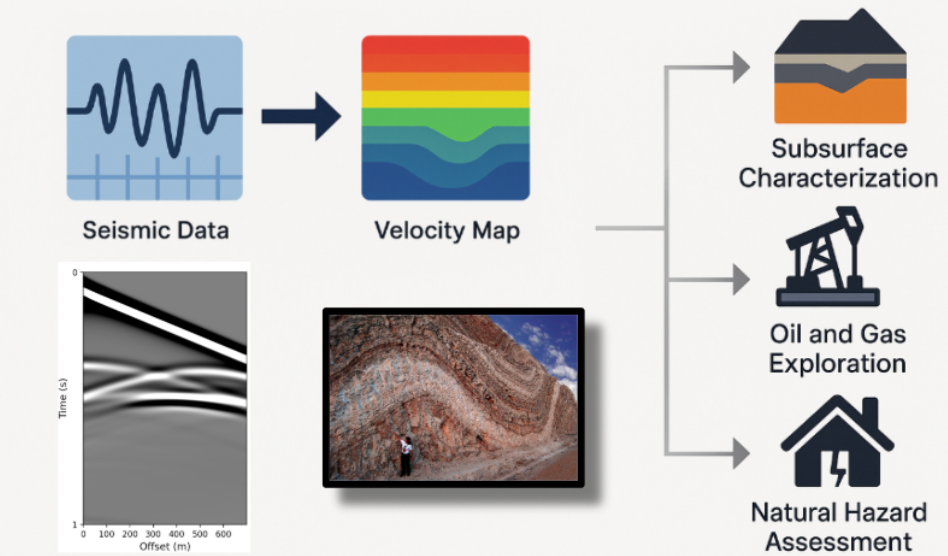
\includegraphics[width=0.5\linewidth]{figures/intro2.png}
        \caption{Velocity Map Formation and its Practical Uses }
        \label{fig:intro2}
    \end{figure}
    
    Unfortunately, however, the placement of receivers underground poses two glaring issues. First and foremost, it is extremely expensive to do, not too different from the cost and manpower it takes to install underground power lines. Second, placing receivers underground may disrupt the subterranean environment that may need to be carefully preserved based on the context. In a hypothetical example, its possible that waveform inversion may be used to detect underground burrows of moles to predict their population. However, installing receivers may destroy these tunnels as a result \cite{ctbto_waveform}.  

    Fortunately, it is possible to install receivers that collect seismic data above ground. They instead capture the reflections of seismic waves to see what is underground, but this method is extremely noisy.   

    \begin{figure}[H]
        \centering
        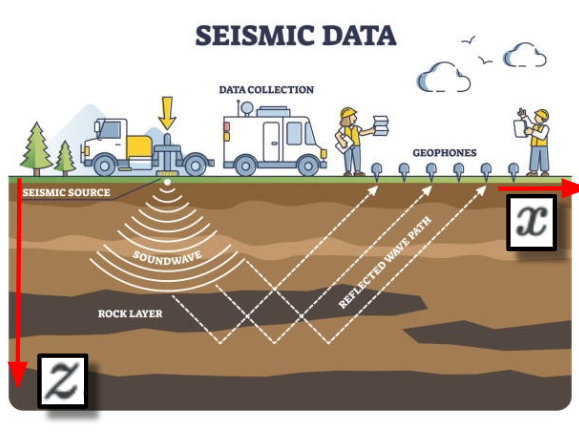
\includegraphics[width=0.5\linewidth]{figures/intro1.png}
        \caption{Collection of Seismic Waveform Data via Above-Ground recievers }
        \label{fig:intro1}
    \end{figure}

    Our work involves using machine learning methods to predict these velocity maps via data from the seismic waves and receiver reflections using several different models. In this study, we employ the following six machine learning models: 

    \begin{itemize}
        \item Fourier Deep ONet
        \item Residual UNet 
        \item InversionNet + VelocityGAN 
        \item 2D Fourier Neural Operator
        \item Augmented Neural ODE 
        \item PCA Dimensionality Reduction
    \end{itemize}

    Of these models, the best performing was Fourier Deep ONet, which achieved a Mean Absolute Error (MAE) of 59.54 on the validation set. At time of writing we are currently 591th place in a Kaggle competition of approximately \~ 1000 people. 

    Each person has made the following contributions: 

    \begin{itemize}
        \item Harini Gurusankar - 
        \item Ryan Irwandy - Worked on the PCA dimensionality reduction MLP Model. 
        \item Girish Krishnan -
        \item Yash Puneet - 
    \end{itemize}

    


\section{Related work} 

    In addition, PCA has been performed before to geographical waveform inversion problems. Specifically in the domain of classifying gas hydrates through a unsupervised neural network model known as Self Organizing Maps (SOM). More specifically, the data's dimensionality is reduced via PCA and then fed into an SOM to cluster different gas hydrates underground \cite{jones2023waveform}.  

    \begin{figure}[H]
        \centering
        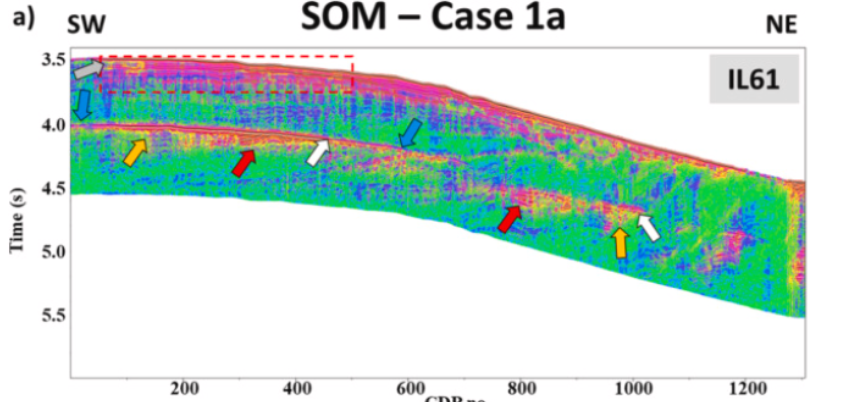
\includegraphics[width=0.5\linewidth]{figures/related1.png}
        \caption{PCA-SOM to classify Gas Hydrates Underground}
        \label{fig:related1}
    \end{figure}
    
    However this problem is a classification problem, and our goal is to predict, specifically, velocity data. However PCA still remains a very good way of reducing dimensionality via principal components while still retaining the variability of our dataset.


\instructions{Related works [5\%]: Please review the related work in this area, state the challenges/limitations of the existing methods, and how does your proposed work will help address the prior limitations and/or advance the current state-of-the-art for this problem.}

\section{Methodology}
\instructions{Method/Approach [40\%]: this should be the main section of your report. Describe your approach, any equation and/or algorithm you developed to solve the problem. This part will be evaluated based on both scientific merit and technical depth.} \\
For this project, a subset of the OpenFWI dataset is used to test the various models, and the best-performing model is then run on the entire dataset (622 GB) for the Kaggle competition. Initially, seismic data is given with dimensions (500, 5, 1000, 70). The description for each dimension is provided below:
\begin{itemize}
    \item 500: The original batch size
    \item 5: The number of seismic sources
    \item 1000: The number of timesteps
    \item 70: The number of receivers
\end{itemize}
The data is then preprocessed by normalization for certain models and then splitting the dataset by batch size into training, testing, and validation sets. After the data is processed, it is passed to a model, which outputs a 70 by 70 velocity map. This velocity map is then compared to a ground truth velocity map and metrics are computed. The metrics chosen for analysis are as shown below:
\begin{figure}[H]
    \centering
    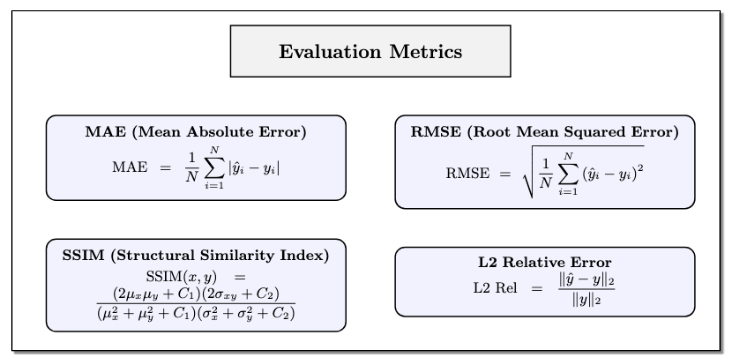
\includegraphics[width=0.5\linewidth]{figures/eval_metrics.png}
    \caption{Formulas for chosen metrics}
    \label{fig:eval-metrics}
\end{figure}
\begin{itemize}
    \item MAE (Mean Absolute Error): This is the base metric for the Kaggle competition.
    \item RMSE (Root Mean Squared Error): This metric adds penalty to larger errors and provides a holistic view when analyzed along with MAE.
    \item SSIM (Structure Similarity Index Measure): This metric is used as a quantitative measure to compare the similarities between a predicted and ground truth image.
    \item L2 Relative Error: This metric is used to measure the difference between predictions and ground truth by accounting for the magnitudes of the values.
\end{itemize}
\subsection{Models}
\subsubsection{Neural ODE}
\begin{figure}[H]
    \centering
    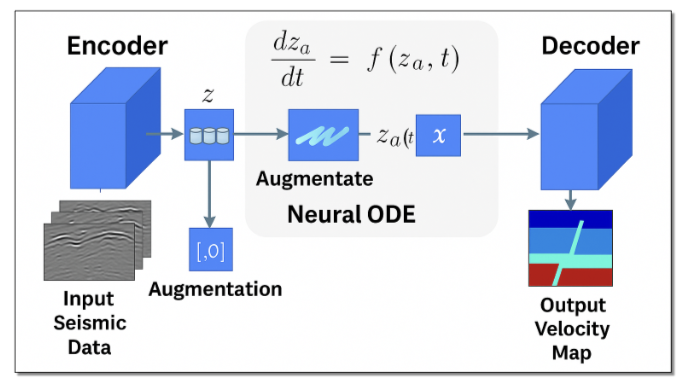
\includegraphics[width=0.5\linewidth]{figures/neuralode_structure.png}
    \caption{Augmented Neural ODE General Structure}
    \label{fig:neuralode_structure}
\end{figure}
One of the models chosen to experiment with was the Neural ODE as learned in the course. Neural ODEs are differential equation solvers, with the solver essentially being a black-box. The model can be implemented by using the torchdiffeq package in Python and the function odeint from this package. The structure of this model was a convolutional encoder, a three-layer MLP as the base function, and a decoder to shape the output as a 70 x 70 tensor to compare against the ground truth. Two different Augmented Neural ODEs were also created. One model had the same MLP as a base function and the other had a simple convolutional network as its base. Both models had an augmented dimension of 1. Augmented Neural ODEs were chosen because the augmented dimension helps in cases where an extra dimension is needed so that trajectories do not intersect. As can be seen in \textbf{Figure 2}, the input seismic data is passed into an encoder and then augmented. This augmented data is passed into the differential equation solver and then decoded into the output velocity map. In \textbf{Figure 3}, the more specific structure of the Augmented Neural ODE with the MLP base is illustrated for further information.
\begin{figure}[H]
    \centering
    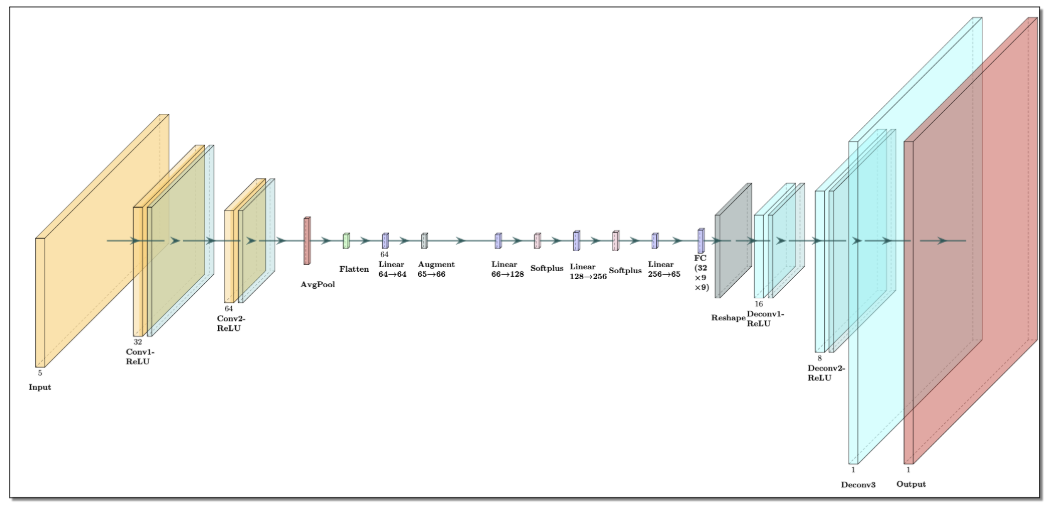
\includegraphics[width=0.5\linewidth]{figures/augmented_neuralode.png}
    \caption{Augmented Neural ODE (MLP)}
    \label{fig:aug-neuralode-mlp}
\end{figure} 

\subsubsection{PCA-MLP} 

To perform Principal Component Analysis (PCA), one must first normalize the data. The most common method of doing so is via Z-Score Normalization: 
 \\
 \\$\frac{x-\mu}{\sigma}$ \\
 \\$\mu$ = Mean\\  
 \\$\sigma$ = Standard Deviation\\ 
 \\$x$ = Datapoint\\ 
 \\ 
The reason for normalizing the data is so features with inherently larger magnitudes do not overshadow those with smaller magnitudes. An example of this is contrasting the number of molecules in a human which is several orders of magnitude larger than human height in inches. 

After performing normalization, we perform PCA analysis by calculating the eigenvectors of the following formula: 
 \\ 
 \\$CV=LV$\\
 \\$C$ = Covariance Matrix\\  
 \\$V$ = Eigenvectors (Principal Components)\\ 
 \\$L$ = Eigenvalues (Loading Scores)\\ 
 \\  
Where $C$ represents the matrix of covariances of each feature against each other, while $L$ and $C$ represent the loading scores and principal components respectively. 

The principal components are computed by calculating an eigenvector of "best fit" that goes through all datapoints represented by $n$ features. The number of eigenvectors calculated is usually up to the number of eigenvectors that describes 95\% of the variability in the dataset as described by the loading scores. Each eigenvector will be perpendicular to the last. The weights that make up an principal component (PC) are known as loading scores, and describe how much a given PC accounts for the variability in a dataset. The PCs now act as the new dependent variables instead of our features.
\begin{figure}[H]
    \centering
    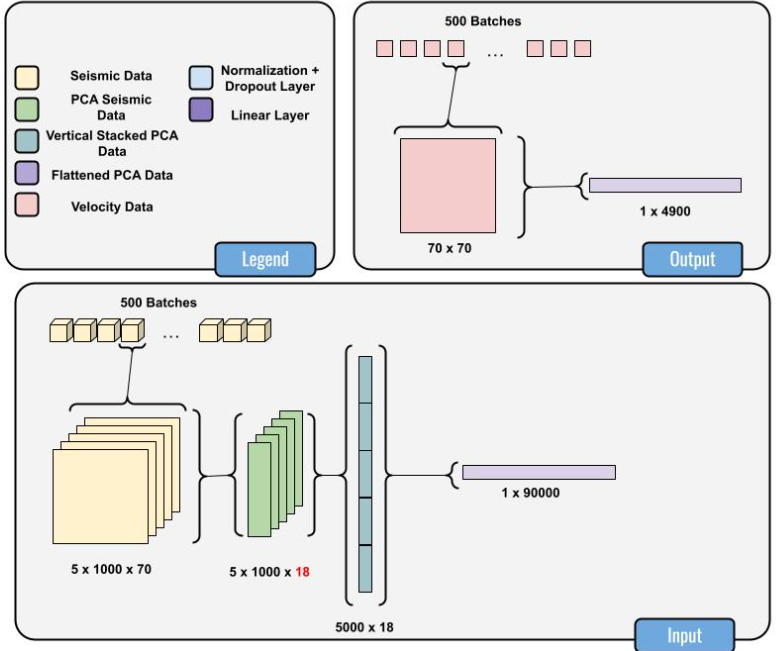
\includegraphics[width=0.5\linewidth]{figures/PCA1.png}
    \caption{PCA Data Preparation}
    \label{fig:pca1}
\end{figure}  
PCA is performed on the seismic waveform dataset by first taking a single batch, which is of dimensions 5 x 1000 x 70. We then further subdivide the data for each source, resulting in a 1000 x 70 matrix where each column represents a given receiver. Because there are so many receivers, we would like to reduce this dimension since its possible that they may be providing redundant data. We reduce this dimension from 70 receivers to 18 PCs. This is partially explained by empirical testing that showed that 18 PCs regularly captured 95\% of the variance for a given source. In addition, we choose a constant number of PCs instead of the minimum number required to capture 95\% of the variance in order to be able to stack each source's PCA data on top of each other, resulting in a 5000 x 18 matrix. Finally we flatten this matrix, which is our new representation of the batch. We then stack every batch on top of eachother and this serves as the input for our model.  

\begin{figure}[H]
    \centering
    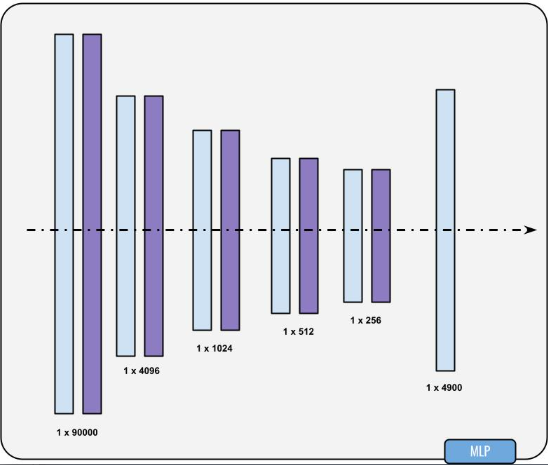
\includegraphics[width=0.5\linewidth]{figures/PCA2.png}
    \caption{PCA-MLP Architecture}
    \label{fig:pca2}
\end{figure}   

The data then gets fed through an MLP, each with its own normalization and dropout layers.


\section{Experiments}
\instructions{Results [30\%]: present your results and provide sufficient discussions of the results. 1) Describe what dataset is being used, details in data processing, train-test data split, and hyperparameter choices in your model etc. Provide the sufficient details such that if a reader would like to reproduce your results, they have enough information to do it. 2) Include figures and/or tables showing the quantitative and qualitative performance of your method; 3) Comparison to necessary baseline methods and comparison to your proposed method.} 

\section{Conclusion}

\subsubsection{Future Work}

For future improvements, we aim to attempt the following with the goal of improving the performance of our project Full Wave Inversion tasks in general as well as in the Kaggle Competition we are submitting to.

\begin{itemize}
    \item \textbf{Evaluate Performance with Noisy Data} In real world scenarios; clean, noise-free data can not always be expected as an input to a model since this is greatly dependent on sensor quality and environmental conditions, thus a model's robustness when faced with noise plays a major role in its overall performance. The Fourier DeepONet Paper [TODO:Reference] performed similar evaluations with InversionNet, VelocityGAN and Fourier DeepONet finding that the DeepONet retained good performance even with noisy data thus we would be interested in comparing our models using a similar process and tuning each model to be as robust as possible to noisy inputs.
    \item \textbf{Hyperarameter Tuning and Larger Dataset for Overfitting Prevention} Through a multitude of experiments as described in Section 4, we found that all of our models overfit the training data to varying extents indicating that model performance could be improved with better tuning or more data. Due to hardware resource and time restrictions we trained our models on a very small subset of the FWI Dataset for the purpose of this project and thus would be interested in evaluating our models on the full dataset with better tuned models. We have currently trained only the Fourier DeepONet with the full dataset. 
    \item \textbf{Dimensionality Reduction with more complex models} Dimensionality Reduction with an MLP backbone worked fairly well in our experiments though its performance was not comparable to our more complex models. Seeing the promise of dimensionality reduction however, we are interested in applying this technique with more our complex models as the backbone to see what performance improvements we can see and potentially reduce overfitting. one such implementation is a PCA-CNN model, as we think it would perform much better since it would retain it's 2D structure instead of losing it when doing PCA.
    \begin{figure}[H]
    \centering
    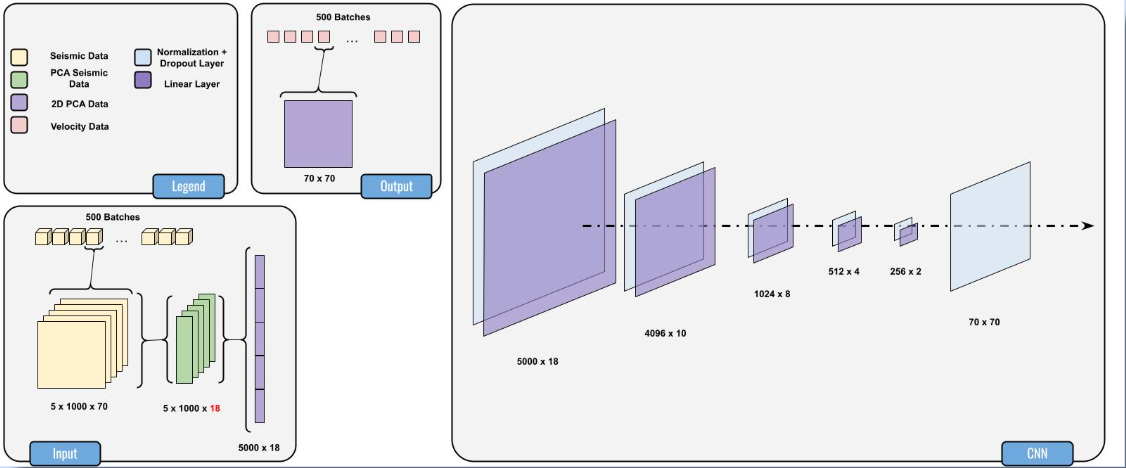
\includegraphics[width=0.5\linewidth]{figures/conclusion1.png}
    \caption{PCA-MLP Architecture}
    \label{fig:conclusion1}
    \end{figure} 
\end{itemize}


\instructions{Conclusion [5\%]: Summarize your project and findings. High-level discussion about what you have learned from this project, what works, and what does not work, and ideas/suggestions for future work if you/others want to work on this problem.} 



\newpage
\instructions{The following sections do not count towards the 8-Page Limits.}
\section*{Appendix}
\subsection*{Github Link}
\instructions{Github Link [10\%]. Include a Link to your Project Github with your project codes with necessary documentation. Please include a top-level README.md file in your github repo. This top-level README should explain the layout of this repository and instructions such that users can run your code. Ensure your code can run and reproduce the results you presented in the report. Note that it is your responsibility to ensure that the code repo is working and the README.md is clear to follow.}

\subsection*{Team Member Contribution}
\instructions{Describing each team member's contribution for this project (e.g., conceptualization, Data curation, Methodology, Software/Experiments, Report Writing, Poster preparation, etc)} 

\bibliography{bib}
\bibliographystyle{abbrvnat}








\end{document}
